\section{Topologie}\label{sec:archi-topologie}
\renewcommand{\rightmark}{Topologie}

Cette section décrit et motive la topologie et les types de noeuds du réseau de capteurs hybride IEEE 802.15.4-LoRa. Cette topologie a été choisie pour correspondre au mieux au cas d'utilisation décrit dans l'introduction.\todo{REF INTRO + à savoir ...}

\subsection*{Types de noeuds}
    Le protocole élaboré pour ce réseau hybride définit 3 types de noeuds:
    \begin{itemize}
        \item[-] La \textbf{racine LoRa} est la passerelle entre le réseau et un réseau IP externe. Elle possède donc une interface LoRa et par exemple une interface Wi-Fi, Ethernet ou 3G/4G.
        La radio LoRa est toujours allumée car ce noeud n'est pas contraint en énergie.  
        \item[-] Les \textbf{racines RPL} sont les racines des réseaux RPL. Elles possèdent une interface LoRa pour communiquer avec la racine LoRa et une interface 802.15.4 pour communiquer avec les noeuds du réseau RPL.
        \item[-] Les \textbf{noeuds RPL} sont des noeuds des réseaux RPL.
    \end{itemize}

\subsection*{Topologie}
Comme l'illustre la figure~\ref{fig:archi-topologie} la topologie choisie est une topologie mixte.

On a d'abord un ensemble de réseaux RPL possèdant chacun un préfixe de sous-réseau IP attribué par la racine LoRa (par exemple $0x02$ ou $0x04$ sur la figure~\ref{fig:archi-topologie}), dans lesquels les communications se font par IEEE 802.15.4.
Comme RPL est utilisé, chaque réseau forme un DODAG.

Ensuite, chaque réseau RPL est connecté à la racine LoRa via sa racine RPL. Les liens entre les racines RPL et la racine LoRa forment une topologie en étoile.

%Ce choix de topologie offre plusieurs avantages: Le fait d'avoir un ensemble de réseaux RPL %implique qu'il n'y a pas qu'une seule racine RPL et donc pas qu'un seul point de défaillance; %L'administration du réseau est également simplifiée. En effet, un réseau RPL pourrait, par exemple, %correspondre à une parcelle de terrain.

Ce choix de topologie a comme avantage de simplifier l'administration du réseau. En effet, un réseau RPL pourrait, par exemple, correspondre à une parcelle de terrain. Comme cette topologie est composée d'un ensemble de réseau RPL, la défaillance d'une racine RPL pourrait impliquer la déconnexion d'un réseau RPL, contrairement à une topologie qui utilise un seul réseau RPL où la défaillance de la racine pourrait impliquer la déconnexion de l'ensemble des noeuds.

L'inconvéninent de cette topologie est que la racine LoRa constitue un seul point de défaillance. Une solution plus robuste qui a été envisagée, est un réseau maillé pour les communications LoRa. Cependant, une telle architecture est difficile à mettre en oeuvre car le protocole MAC a établir pour les liens LoRa est plus complexe et nécessite un protocole de routage.

\begin{figure}[H]
    \centering
    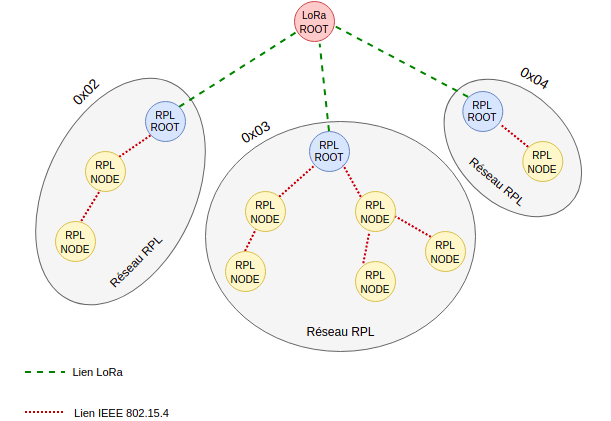
\includegraphics[scale=0.7]{res/pictures/loramac-topologie.drawio.png}
    \caption{Topologie du réseau hybride.}
    \label{fig:archi-topologie}
\end{figure}

%Ainsi, l'objectif de cette topologie est de transmettre les paquets IP à destination de la racine %LoRa.

L'essentiel du travail consite donc à définir et mettre en place un protocole MAC utilisant LoRa pour les communications entre les racines RPL et la racine LoRa ainsi que les mécanismes permettant de passer d'un réseau à un autre. Le routage est le transfert des paquets dans les réseaux RPL est quand à lui assuré par RPL et IPv6. Les sections suivantes décrivent le protocole MAC mis en place pour les communications LoRa.